\documentclass[12pt,english]{article}
\usepackage{lmodern}
\linespread{1.05}
%\usepackage{mathpazo}
%\usepackage{mathptmx}
%\usepackage{utopia}
\usepackage{microtype}
\usepackage[T1]{fontenc}
\usepackage[latin9]{inputenc}
\usepackage[dvipsnames]{xcolor}
\usepackage{geometry}
\usepackage{amsthm}
\usepackage{amsfonts}

\usepackage{courier}
\usepackage{verbatim}
\usepackage[round]{natbib}
\bibliographystyle{plainnat}

\definecolor{red1}{RGB}{128,0,0}
%\geometry{verbose,tmargin=1.25in,bmargin=1.25in,lmargin=1.25in,rmargin=1.25in}
\geometry{verbose,tmargin=1in,bmargin=1in,lmargin=1in,rmargin=1in}
\usepackage{setspace}

\usepackage[colorlinks=true, linkcolor={red!70!black}, citecolor={blue!50!black}, urlcolor={blue!80!black}]{hyperref}
%\usepackage{esint}
\onehalfspacing
\usepackage{babel}
\usepackage{amsmath}
\usepackage{graphicx}

\theoremstyle{remark}
\newtheorem{remark}{Remark}
\begin{document}
	
		Employee spinouts can be a key driver of productivity growth, but they can also disincentivize innovation ex ante when firms anticipate they will compete with them [NEED TO TALK ABOUT EX ANTE VS EX POST]. A common solution is a non-compete contract (NCC), which legally precludes the employee from competing with her previous employer. However, some states -- in particular, California -- have achieved high rates of productivity growth while refusing to enforce such contracts, and scholarly work thus far has been inconclusive (fix this -- deosn't link to anything). In this paper, I study the effect of competition by employee startups on productivity growth, with an application to the optimal enforcement of covenants not to compete. To do so, I first develop a fully dynamic general equilibrium model of endogenous growth in which R\&D employment by incumbents leads to the formation of spinouts. The model implies that easier employee spinout formation has a non-monotonic effect on growth and welfare: first increasing it but eventually decreasing it by disincentivizing innovation (this sentence is kind of unclear. Try to explicitly talk about the two channels -- more creative destruction, more disincentive -- and then talk about how one eventually dominates). To discipline the model, I construct and analyze a new dataset combining several micro-level datasets: (1) proprietary data on VC-funded startups and their founders, data on R\&D and stock prices (4) patent data for public firms from the NBER-USPTO database (is this too standard to name? looks pedantic), and (5) firm-specific instruments for R\&D expenditure based on subsidies (from \cite{bloom_identifying_2013}). I use the resulting dataset to calibrate the theoretical model's parameters. The model's predictions across NCC enforcement regimes (states? clarify) can be compared to those in the data. Finally, I use the model to study the growth and welfare effects of NCC enforcement and R\&D subsidies. The calibration suggests XYZ.
		
		
		
		\begin{itemize}
			\item Do I need clarification in first sentence. Also avoid parentheses and reread Cochrane's thing
			\item Call them non-competes not CNCs 
			\item Data section: emphasize proprietary + complementary standard data (bucket with everything else). simpler, less pedantic
			\item Get rid of citation to Bloom -- also, this could be in the methodology section, and avoids having to include this in the data section 
			\item Empirical methodology kind of clear
			\item Results scattered across abstract -- try to put all in the end 
		\end{itemize}
		

\textbf{Notes from Ezra and Moll:}

\begin{itemize}
\item Moll: get to point faster (see Research Proposal you submitted recently for a shorter version of introduction.
\item Ezra: reduce emphasis on comparing to similar work. just say what you did. also, be gentle when discussing other work. This is VERY important - people will be reviewing your work - be generous (more than already!
\end{itemize}

\textbf{How do I join the conversation?}

\textbf{What is my motivation?}

\begin{itemize}
\item Previous empirical papers are iconclusive
\item And specifically, previous modeling isn't the right way to model 
\item The theory is very important, because we are talking about contracting (but can I do a good job on this??)
\end{itemize}

\textbf{What are my contributions?}

\begin{itemize}
\item Constructing new data set
\item Documenting new empirical facts about relationship of R\&D spending flow and spinout formation (controlling for patent stocks)
\item Constructing new model with interesting mechanisms in it (e.g. "escape competition effect"), yet somewhat tractable
\end{itemize}
\section{introduction}


Silicon Valley (SV) is often hailed as a paragon of economic dynamism and innovation. And not without reason: labor productivity growth in the MSA containing SV averaged 2.72\% from 1978 to 2015, compared to an average of about 2\% for the whole country. This difference in growth rates implies a 30\% increase in the level of productivity over the time period, which likely underestimates the contribution to aggregate labor productivity growth for several reasons. \footnote{See \cite{parilla_understanding_2017}. Further, the employment growth rate exceeded the national average during this time period, increasing the contribution to aggregate labor productivity growth. Even more importantly, labor productivity growth in SV has been centered on ICT-producing firms, whose output contributes heavily to labor productivity growth in other industries. \cite{jorgenson_retrospective_2008} attributes nearly half of labor productivity growth from 1973-2006 (and more 60\% from 1995-2000) to ICT. Consistent with this, the appendix of  \cite{parilla_understanding_2017} reports that labor productivity growth peaked at almost 5\% annualized in the MSA containing SV from the years 1994-2005.} The literature has argued for the importance of employee mobility and entrepreneurship in the region, with a particularly important part played by \textit{employee spinouts}: firms founded by former employees in the same or related industries as the former employer. \footnote{See \cite{saxenian_regional_1994}, \cite{gilson_legal_1999}, \cite{fallick_job-hopping_2006}, \cite{franco_covenants_2008}.} \footnote{This is different from a "spinoff", which is a division of a firm that the firm itself decides to sell. The early literature uses these terms interchangeably, but the more recent literature has settled on the term "spinout" for entrepreneurship initiated by the employee.} As an anecdotal illustration, Figure \ref{fairchild_spinouts} shows the many direct and indirect spinouts of Fairchild Semiconductor, one of the first leading semiconductor firms of SV -- itself a spinout of Shockley Laboratories, another semiconductor firm. Although Fairchild was founded in the 1950s, its list of spinouts includes some of the most well-known modern firms in SV, such as Intel and AMD. In turn, the literature has hypothesized that SV's unusual rates of employee mobility and entrepreneurship are due to California's prohibition on the enforcement of covenants not to compete (CNCs). \footnote{\cite{saxenian_regional_1994} attributes SV's rise from the 1960s to the 1990s (relative to Route 128 in Massachusetts, the previous tech hub) to SV's higher degree of employee mobility and entrepreneurship, as well as to its modular industrial structure. In turn, \cite{gilson_legal_1999} argues that this resulted from California's state-level statue not to enforce a labor contract known as a covenant not to compete (CNC), or simply non-compete.  \cite{fallick_job-hopping_2006} complements this view using survey data from the CPS, providing evidence that employee mobility is (1) higher in the computer industry in SV than in computer industries in other regions, and (2) higher in the computer industry in California than in the computer industries outside of California. The authors interpret this as evidence of a California-level factor rather than something SV-specific, and suggest an interpretation in line with the hypothesis of \cite{gilson_legal_1999}. Finally, \cite{franco_covenants_2008} considers a two-region model of spinout formation with and without CNCs in which the enforcing region has more initial firm entry but is eventually overtaken by the non-enforcing region.} Such contracts prevent departing employees from joining or founding competing firms for a span of time (usually 6 months to 2 years) and often in a certain geographical region. Figure \ref{noncompetes_enforcement} illustrates the state-level cross-sectional variation in the degree of enforceability of such contracts. California's lack of enforcement is far from typical.

\begin{figure}	\phantomsection
	\center
	\includegraphics[scale = 0.77]{../figures/fairchildren_early.png}
	\caption{Direct and indirect spinouts of Fairchild Semiconductor}
	\label{fairchild_spinouts}
\end{figure}

\begin{figure}	\phantomsection
	\center
	\caption{State-level enforceability of CNCs. Source: Bishara 2011}
	\includegraphics[scale = 0.68]{../figures/noncompetes_enforcement.png}
	\label{noncompetes_enforcement}
\end{figure}



Of course, the specific cause of SV's rise is difficult to ascertain. Nevertheless, the preceding question motivates the general question of what effect spinout entrepreneurship -- and in particular enforceability of non-competes -- has on innovation and labor productivity growth. This paper attempts to take a step towards answering this question.



Several strands of the literature point to the importance of answering this question. A large literature that has argued for the importance of business entry in labor productivity growth.\footnote{Using an accounting decomposition, \cite{foster_aggregate_2001} estimates that entry accounts for 25\% of aggregate productivity growth in the United States. See \cite{brandt_creative_2012} for evidence from China. See \cite{asturias_firm_2019} for evidence from Chile and Korea. \cite{akcigit_growth_2018} arrives at a similar estimate using a structural approach disciplined by patent citations data.} Another empirical literature has documented that employee spinouts are more productive, grow faster, and survive longer than other entrants.\footnote{See \cite{baslandze_spinout_2019} for evidence from US patent data and Compustat. See \cite{muendler_employee_2012} for evidence from Brazilian employer-employee matched data.} A related literature has argued that spinouts inherit knowledge from their parents, and that parent firms tend to be productive and knowledge intensive.\footnote{See \cite{klepper_entry_2005}, \cite{gompers_entrepreneurial_2005}, and \cite{baslandze_spinout_2019}.} 

\textbf{[need to distinguish between competing spinouts and non-competing spinouts. this part needs to be reworked.]}
Theory suggests that the answer to this question is non-trivial. As pointed out by Schumpter, \cite{arrow_economic_1962}, and more recently \cite{romer_increasing_1986}, the limited excludability of knowledge means the returns to investment cannot be fully appropriated. If CNC enforcement reduces the formation of spinouts, incumbent firms can better appropriate the returns of knowledge (or capital) investments. By increasing appropriability, CNC enforcement induces more investment by incumbent firms in equilibrium. CNCs play a role similar to patents, which also incentivize investment in knowledge by reducing knowledge spillovers and competition.

However, note that in the case of employee spinouts, the employee can only appropriate the firm's investments because of his contractual relationship with the employer  (i.e., because he working for her).  Therefore, as highlighted by \cite{franco_spin-outs:_2006}, incumbent firms will be compensated for this lost value in the form of lower equilibrium wages. This occurs due to employees pricing in the value of the know-how they acquire on the job. In that model, even without CNC enforcement, the equilibrium is Pareto efficient. A crucial assumption, though, is that spinouts do not compete directly with the parent firm. If they do, the potential to form a spinout reduces the bilateral value of the firm and employee. The effective wage paid by the firm -- taking into account the potential lost value from competition -- is higher than if there were a CNC. This reduces the incentive to invest in knowledge. 

On the other hand, even if CNCs allow incumbent firms and their employees to write a bilaterally more efficient contract, incumbents will in general still underinvest in R\&D relative to the social optimum due to monopoly power. Forcing them to allow spinouts may increase efficiency by increasing knowledge diffusion and producing firms motivated by creative destruction. Such firms invest a socially excessive amount in R\&D due to business-stealing, which may offset the underinvestment by incumbent firms.\footnote{This is one of the insights from the literature spawned by \cite{grossman_quality_1991}. In the basic models, the effect of business stealing on equilibrium innovation rates is stark: incumbent firms are entirely priced out of innovation by firms attempting creative destruction.}

Finally, politically, there is a significant amount of momentum towards limiting the enforcement of CNCs, both at the federal and state level. In 2015 Hawaii banned non-competes for technology workers. In 2018, Massachusetts passed legislation significantly limiting the scope of enforceable CNCs. Other states have recently made similar proposals.\footnote{See \cite{the_white_house_technical_report_non-compete_2016}.} In light of this, there is an urgent need to improve our understanding of the issue. 

\paragraph{Related literature}

Some work has attempted to answer this question directly using empirical methods. Papers in this literature have typically used either cross-sectional and/or longitudinal variation in the state-level enforcement of non-competes.\footnote{Sometimes this variation is argued to be exogenous, either due to legislative error as in \cite{marx_mobility_2009} and \cite{marx_regional_2015}, or due to unexpected judicial precedent as in \cite{jeffers_impact_2018}. Often there is a control industry that is believed to be unaffected by the variation in CNC enforcement policy (e.g. law firms are typically exempt from CNC restrictions).} The results are inconclusive and suggest an important tradeoff between entry of spinouts and investment by incumbent firms. \cite{stuart_liquidity_2003} find more local  entrepreneurship in response to local IPO (a "liquidity event") in regions not enforcing CNCs. \cite{marx_mobility_2009} finds that inventor mobility declines in response to an increase in non-compete enforcement. \cite{samila_venture_2010} finds that an increase in VC funding supply increases entrepreneurship more in states without non-compete restrictions, using an IV design. \cite{garmaise_ties_2011} finds that, in states where CNCs are more enforceable, managers are less mobile, have lower compensation, and invest less in their human capital, to the point of offsetting increased investments by the firm. On the other hand, \cite{conti_non-competition_2014} finds evidence that non-compete enforceability leads to incumbent firms pursuing riskier R\&D projects. \cite{colombo_does_2013} finds evidence that easier spinout formation -- proxied by access to finance -- leads to a reduction in incumbent firm knowledge investments.  Most recently, \cite{jeffers_impact_2018} uses data on influential state-level court precedents matched with LinkedIn data and finds that enforcement indeed reduces spinout formation while increasing capital investment by incumbent firms. Finally, \cite{marx_regional_2015} finds that CNC enforcement leads to inventor mobility out of the state, suggesting that differences in outcomes could be in part due to reallocation. 

Theoretical work has also explored this question. As mentioned previously, \cite{franco_spin-outs:_2006} develops a model in which employees learn from their employers and use this knowledge to form spinouts. They emphasize the "paying for knowledge" effect, whereby employees implicitly pay for the knowledge they take from the parent firm through lower equilibrium wages. Importantly, they assume spinout firms do not steal business from their parents: the only effect of a spinout on the parent firm is a reduction in the price of the output good, which the parent firm is assumed not to take into account. This, combined with the "paying for knowledge" mechanism, ensures that the competitive equilibrium allocation is Pareto efficient, even without resorting to elaborate labor contracts.

\cite{franco_covenants_2008} studies a two-period, two-region model with employee spinouts in which the region which does not enforce CNCs initially lags but eventually overtakes the region in which CNCs are enforced. In the first period, entry is more valuable in the enforcing region. But in the second period, spinouts enter in the non-enforcing region, there is Cournot competition with parent firms in the product market, and output increases relative to the enforcing region. The analysis emphasizes how asymmetric information about whether an employee has learned leads some firms in the non-enforcing region to allow spinouts (assuming firms cannot commit to wage backloading). This can be taken as a rough microfoundation of my assumption that labor contracts are "simple" in  a non-enforcing region: just a wage, with no attempts at retention in the case of learning. They do not consider long-run growth implications, and use a two period model. Spinouts do not worry about spinouts of their own. R\&D is not present - only entry in the first period leads to a certain chance of spinout formation in the second period. 

\cite{shi_restrictions_2018} uses a rich model of contracting disciplined by data on executive non-compete contracts to study the effect of non-competes on executive mobility and firm investment. She finds that the optimal policy is to somewhat restrict the permitted duration of CNCs. Her approach allows her to study the optimal contracting problem in more detail than in mine. However, she is mainly interested in poaching, which involves an attempt to extract a payout from the poaching firm, while I am interested in spinouts. Also, her calibration relies heavily on matching the response of firm investment to the presence of a CNC in the manager's contract. However, she uses capital investment rather than investment in knowledge. This leads her to estimate an R\&D elasticity such that non-competes do not do much to increase the incentives for firm investment. However, I am interested in long-run growth, which is driven by investments in knowledge (in the data, R\&D not capex).

\cite{baslandze_spinout_2019}, the study closest to this paper, studies the effect of spinout entrepreneurship on entry and growth. Baslandze's analysis concludes that the optimal enforcement of non-competes is zero. However, in her framework, spinouts do not steal business from the parent firm, instead entering into a different product line. The harm to the parent firm results from the additional assumption that the parent firm's technology gap -- relative to potential entrants in its own product-line -- drops to zero upon spinout formation. This is modeled as other firms "catching up" technologically to the incumbent, although it is interpreted as the loss of match-specific productivity. In other words, the knowledge of the firm is fully embodied in its R\&D manager. My paper focuses instead on creative destruction of the parent firm using knowledge that is embodied in the firm but can be used simultaneously by the employee in a spinout.  More importantly, in her analysis, higher non-compete enforcement is modeled as a higher cost of spinout formation. This is unsatisfactory because it precludes the possibility that bilaterally efficient spinouts will be allowed even in CNC enforcing regions. 

In addition, the preceding studies are not disciplined by an empirical measurement of the extent to which spinout firms reduce bilateral value, as opposed to simply entering other markets using similar technology. Given the theoretical analysis above, this is critical to the question of whether the decentralized equilibrium is efficient, either with or without elaborate labor contracts. The contribution of this paper is to provide some empirical measurement on this quantity, along with a framework that models its effect on the key outcomes of interest: labor productivity growth and -- taking into account the cost of investment -- the present discounted value of output per person (welfare in my model).



\section{Quantitative analysis (preliminary)}\label{quantitative_analysis}

In this draft, I analyze the implications of the model given a preliminary calibration not based on the micro-data I will use in the final version.

\subsection{Calibration}

Table 1 displays the parameter values used in the preliminary calibration, as well as broadly how they are identified.

\begin{table}[h]
	\centering{}%
	\begin{tabular}{lll}
		Table 1 &  &  \tabularnewline
		Calibration Parameters &  &  \tabularnewline
		\hline 
		Parameter & Explanation & Value\tabularnewline
		\tabularnewline
		\hline 
		Normalized & & \tabularnewline
		$\xi$ & Spinout R\&D capacity & 10 \tabularnewline
		&  & \tabularnewline
		Chosen outside model & & \tabularnewline
		$\psi_I$ & Incumbent R\&D curvature & 0.5\tabularnewline
		$\psi_E$ & non-Incumbent R\&D curvature & 0.5\tabularnewline
		&  & \tabularnewline
		Chosen to match data & & \tabularnewline
		$\rho$ & Discount rate & 0.05\tabularnewline
		$\beta$ & $\beta^{-1}$ is EoS between intermediate goods & 0.106\tabularnewline
		$\lambda$ & Innovation step size & 1.053\tabularnewline
		$\chi_I$ & Incumbent R\&D productivity & 3.252\tabularnewline
		$\chi_E$ & Entrant R\&D productivity & 1.203\tabularnewline
		$\chi_S$ & Spinout R\&D productivity & 1.425\tabularnewline
		$\nu$ & Learning rate & 0.0103
	\end{tabular}
\end{table}

Table 2 displays the calibration targets, which parameter(s) they principally inform, and the relevant model-generated moment. For this calibration, I drew heavily from \cite{akcigit_growth_2018}.\footnote{The profit / sales ratio, R\&D spending / sales ratio, and internal patent share are taken from \cite{akcigit_growth_2018} and matched to the analogous model counterparts. The spinout entry rate is equal to the entry rate in that model, so it should be smaller. The share of creative destruction by spinouts is not taken from data - for now, I calibrated it to 30\%, but I will eventually discipline this with data.} The fit of the model to the data is reasonable, although there are as many parameters as moments.

Notice that $\nu,\xi$ are not separately identifiable in this model: their joint impact on the model is summarized entirely through $\nu \xi$. The value $\nu \xi \approx 0.1$ roughly means that over the course of a year of performing R\&D, potential spinouts will form capable of conducting 10\% the parent firm's R\&D effort. However, this is only rough, as it does not take into account the different pools of ideas or the different per-employee R\&D productivity of spinouts. 

\begin{table}[h]
	\centering{}%
	\begin{tabular}{llll}
		Table 2 & & &  \tabularnewline
		Calibration Targets & & &  \tabularnewline
		\hline 
		Moment & Parameter(s) & Target & Model \tabularnewline
		&  &  & \tabularnewline
		\hline 
		Growth rate $g$ & $\lambda$ & 0.015 & 0.0198 \tabularnewline
		Risk-adjusted interest rate $r$ & $\rho$ & 0.05 & 0.05 \tabularnewline
		Profit / sales ratio & $\beta$ & .109 & .109 \tabularnewline
		R\&D spending / sales ratio & $\lambda,\chi_I,\chi_E,\chi_S$ & 0.15 & 0.093
		\tabularnewline
		Internal patent share & $\chi_I / \chi_E$ & 0.2 & 0.202
		\tabularnewline
		Spinout entry rate & $\nu \xi$ & 0.05 & 0.084
		\tabularnewline
		Share of creative destruction by spinouts & $ \chi_S / \chi_E$ & 0.30 & 0.283 
	\end{tabular}
\end{table}

\subsection{Descriptive plots}

First I will show some plots from the equilibrium illustrate the equilibrium that obtains in the above calibration. 

Figure \ref{RD_wages} shows the equilibrium wages and flow value of knowledge transfer from employee learning. The production wage is constant, as expected. The R\&D wage increases over the course of a product's life cycle, as the knowledge earned by the marginal R\&D worker decreases due to more competition by other spinouts in R\&D. The effective R\&D wage incorporates the lost monopoly power of the incumbent; depending on the interplay of these two forces, the effective R\&D wage can be below or above the final goods wage -- which is also the wage that would prevail under a (permanent) non-compete contract.

\begin{figure}[h] \phantomsection 
	\centering
	\includegraphics[scale=0.5]{../code/julia/figures/presentation/plot_effectiveRDWage_vs_t.png}
	\caption{The top panel shows the equilibrium production wage (blue), R\&D wage (yellow) and effective R\&D wage (red). The effective R\&D wage increases over the life-cycle of a quality-level of a product. The bottom panel shows the flow expected value of knowledge transfer, from the perspective of the R\&D worker (yellow), the incumbent (blue) and the coalition of the incumbent and the R\&D worker (red). As in the theoretical discussion, when the flow expected value to the coalition is negative, the effective R\&D wage exceeds the final goods wage, which is the wage that would prevail under a non-compete.}
	\label{RD_wages}
\end{figure}


Figure \ref{innovation_rates} shows the equilibrium arrival rates of innovations over the life-cycle of a product (i.e. as a function of the time since the last innovation). Two things are noteworthy. First, potential spinouts gradually replace potential entrants. Second, the incumbent's R\&D intensity increase significantly over the course of a product's life cycle. Since the effective R\&D wage is increasing and the reward from innovating is constant, this quite dramatic effect is entirely due to the "escape competition" effect. In fact, the figure suggests that approximately 60\% of the variation in product replacement rates over the course of the product-life cycle is due to variation in the incumbent's innovation effort motivated by the escape-competition effect.

\begin{figure}[h] \phantomsection
	\centering
	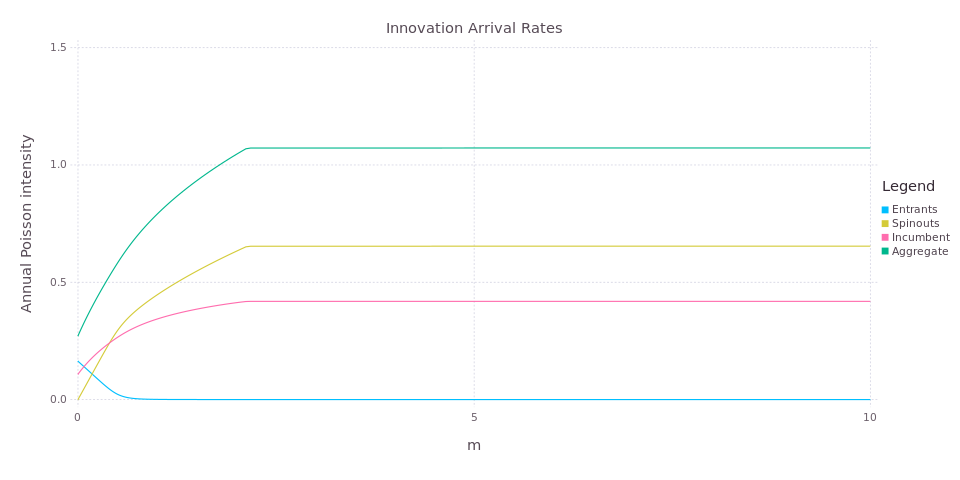
\includegraphics[scale=0.5]{../code/julia/figures/presentation/innovation_rates.png}
	\caption{Above shows the equilibrium innovation (annual) hazard rates over the evolution of a product. The hazard rate of innovation increases as (1) more spinouts enter and (2) incumbents do more R\&D to escape the competition they have created.}
	\label{innovation_rates}
\end{figure}

\subsection{Comparative statics}

Figure \ref{nuxi_chiS_gCompStat} shows the growth implications of varying the rate of employee learning. Equilibrium growth is inverse-U shaped in $\nu \xi$, with a peak shifting to the right as $\chi_S$ is increased. This reflects the tradeoffs discussed in the theory section.

\begin{figure}[h] \phantomsection
	\centering
	\includegraphics[scale=0.5]{../code/julia/figures/presentation/nuxi_chiS_g_plot_2.png}
	\caption{Implications of $\nu \xi$ and $\chi_S$ for the growth rate $g$ and the R\&D labor allocaiton $L_{RD}$. Both effects are non-monotonic, with peaks that are increasing in $\chi_S$.}
	\label{nuxi_chiS_gCompStat}
\end{figure}

Figure \ref{nuxi_growthDecomposition} shows the decomposition of growth and R\&D employment by incumbents, spinouts and entrants as $\nu \xi$ varies, holding $\chi_S$ constant at the calibrated value. The contribution of spinouts to growth increases as $\nu \xi$ increases, while the contribution of ordinary entrants to growth decreases. These largely offset each other. The contribution of incumbents to growth increases at first and then decreases gradually as $\nu \xi$ increases. 

The top panel of Figure \ref{nuxi_growthDecomposition} shows the R\&D employment. Incumbent firms employ less than 1/10 of the R\&D workers as potential entrants (including spinouts), but lead end up with 1/4 of the growth contribution. This is due to the assumptions on the relative R\&D productivity of entrants and incumbents. As this appears to be at odds with the data, this warrants further investigation.

\begin{figure}[h] \phantomsection
	\centering
	\includegraphics[scale=0.5]{../code/julia/figures/presentation/nuxi_RDandGrowth_plot.png}
	\caption{Growth and R\&D spending decompositions. The bottom panel shows the equilibrium growth decomposition as a function of $\nu \xi$. As $\nu \xi$ increases, the incumbent contribution to growth (blue) increases, but eventually it begins to decrease. Non-spinout entrant contribution to growth decreases monotonically as $\nu \xi$ increases, and the reverse is true for the spinout contribution. The top panel shows R\&D labor used by incumbents, entrants and spinouts. The calibration that incumbents are more productive at R\&D than entrants or spinouts means that incumbents can contribute half as much to growth as entrants / spinouts while deploying 10\% of the R\&D labor. This seems at odds with the data, suggesting I may need to modify my model to account for this.}
	\label{nuxi_growthDecomposition}
\end{figure}

Figure \ref{nuxi_chiS_welfare} shows the welfare effects of varying $\nu \xi$ and $\chi_S$. As in the previous comparative statics, welfare is non-monotonic in $\nu \xi$ given $\chi_S$, with a peak that is increasing in $\chi_S$. As noted previously, increasing $\nu \xi$ expands the production possbilities frontier of the economy. Hence, the decrease in welfare is a lower bound on the inefficiency of the model. In the current calibration, peak decentralized welfare is at $\nu \xi \approx 0.4$. Of course, since I have not solved the planner's problem, the equilibrium may very well still be inefficient at this value. 

Finally, inspecting Figure \ref{nuxi_chiS_welfare} shows that the model predicts substantial welfare gains from increasing the calibrated value of $\nu \xi = 0.1$ to $\nu \xi = 0.4$, of approximately 5\%. This may not be a policy instrument available to the policy maker or even social planner, but it suggests that in this range, relaxing restrictions on spinout formation could significantly improve welfare. 

%\begin{figure}[h] \phantomsection
%	\centering
%	\includegraphics[scale=0.5]{../code/julia/figures/presentation/nuxi_chiS_welfare_plot.png}
%	\caption{Welfare implications of varying $\nu \xi$ and $\chi_S$. Welfare is non-monotonic in $\nu \xi$, even though this expands the production possibilities frontier. Peak decentralized welfare is increasing in $\chi_S$.}
%	\label{nuxi_chiS_welfare}
%\end{figure}


	
	
	
	
\end{document}